\documentclass[../main.tex]{subfiles}
\begin{document}
\section{搜索与优化基础}\label{sec:search-optimization}
\subsection{状态空间与搜索树}\label{sec:state-space-search-tree}
\begin{enumerate}
    \item \textbf{状态空间：}利用状态变量和操作符号，表示系统或问题的有关知识的符号体系。
    \begin{itemize}
        \item \textbf{状态空间四元组：}
        \begin{itemize}
            \item $S$：状态集合；
            \item $O$：操作算子的集合；
            \item $S_0$：包含问题的初始状态，是 $S$ 的非空子集；
            \item $G$：若干具体状态或满足某些性质的路径描述。
        \end{itemize}
        \item \textbf{求解路径：}从 $S_0$ 节点到 $G$ 节点的路径。
        \item \textbf{状态空间的一个解：}一个有限的操作算子序列。
    \end{itemize}

    \item \textbf{状态空间图：}把问题抽象为某个有向图中寻找目标或路径的问题，这种描述问题的有向图称为状态空间图，简称状态图。

    \item \textbf{搜索：}为模拟问题求解过程而发展的一种技术，本质上是考虑各种可能的行动序列，通过搜索求解。

    \item \textbf{问题求解智能体设计的基本步骤：}
    \begin{itemize}
        \item \textbf{目标形式化（goal formulation）：}“成功”的状态描述；
        \item \textbf{问题形式化（problem formulation）：}根据所给的目标考虑行动和状态的描述\footnote{往往要将真实复杂情况抽象化，果我们能把任何抽象解扩展成为更细节的世界中的解，这种抽象就是有效的；选择好的抽象，包括：(1)在保持有效抽象前提下去除尽可能多的细节；(2)确保抽象后的行动容易完成；}；
        \item \textbf{搜索（search）：}通过对行动序列代价计算来选取最佳的行动序列；
        \item \textbf{执行（execute）：}给出“解”并执行行动。
    \end{itemize}

    \item \textbf{问题求解智能体的环境特性：}
    \begin{itemize}
        \item \textbf{静态的：}完成问题形式化和求解的时候不再考虑环境可能的变化；
        \item \textbf{可观察的}；
        \item \textbf{离散的：}可枚举“可选的行动”；
        \item \textbf{确定性的：}问题的解是行动的单一序列。
        \begin{itemize}
            \item 不能处理意外事件；
            \item 执行问题的解的过程中也不注意感知信息。
        \end{itemize}
        \item \textbf{属于最简单的一类环境。}
    \end{itemize}

    {\small\kaishu
    \textbf{例：旅行路线问题求解步骤}\footnote{一个智能体有多个评价未知的直接选项的时候，可以首先检验各个不同的能导致已知评价的状态的可能行动序列，然后选择其中最佳的序列。}
    \begin{itemize}
        \item \textbf{问题：}现在在城市A，要到城市B；
        \item \textbf{目标形式化：}$\mathrm{be\ in\ B}$；
        \item \textbf{问题形式化：}
        \begin{itemize}
            \item 状态：在某个城市；
            \item 动作：开车从一个城市到另一个城市。
        \end{itemize}
        \item \textbf{寻找解（搜索）：}动作序列，如：A$\rightarrow$S$\rightarrow$F$\rightarrow$B。
    \end{itemize}
    }
     \item \textbf{良定义的问题及解：}一个问题由 $5$ 个组成部分形式化描述：
    \begin{itemize}
        \item 初始状态；
        \item 可能行动\footnote{初始状态+可采纳的行动=状态空间}；
        \item 转移模型；
        \item 目标测试函数；
        \item 路径耗散（代价、成本）函数。
    \end{itemize}
    问题的环境用状态空间表示，状态空间中从初始状态到达目标状态的路径是一个解。
\end{enumerate}

\subsection{搜索树结构与算法}\label{sec:search-tree-algorithm}
\begin{enumerate}
    \item \textbf{搜索技术：}
    \begin{itemize}
        \item 搜索是人工智能技术中进行问题求解的基本技术\footnote{不管是符号智能还是计算智能，最终往往都归结为某种搜索；图搜索模拟的是人脑分析问题、解决问题的过程；}；
        \item 搜索的主要过程（三要素）：
        \begin{itemize}
            \item \textbf{状态空间（state space）：}从初始或目的状态出发，并将它作为当前状态；
            \item \textbf{后继函数（successor function with actions and costs）：}扫描操作子集，将适用于当前状态的一些操作算子作用于当前状态而得到新的状态，并建立指向其父结点的指针；
            \item \textbf{初始状态和目标测试（start state and goal test）：}解是一个行动序列，将初始状态转换成目标状态。
        \end{itemize}
    \end{itemize}

    \item \textbf{图数据结构与树数据结构：}
    \begin{itemize}
        \item \textbf{图：}
        \begin{itemize}
            \item 图从数学领域进化而来，主要用来描述一个从一个位置到另一个位置的路线的模型；
            \item 一个图包含一系列的点和一系列的边；
            \item 边用来把点连接起来；
            \item 路线（路径）是用来描述共用一条边的点的轨迹的术语。
        \end{itemize}
        \item \textbf{树：}
        \begin{itemize}
            \item 树和图一样也是一系列点的集合；
            \item 有一个根节点；
            \item 这个根节点有一些子节点；
            \item 子节点也有它们自己的孙子节点；
            \item 树是没有环的图；
            \item 一个子节点只有一个父节点。
        \end{itemize}
    \end{itemize}

    \item \textbf{状态图搜索：}
    \begin{itemize}
        \item \textbf{搜索：}从初始节点出发，沿着与之相连的边试探地前进，寻找目标节点的过程；
        \item \textbf{搜索树：}搜索过程中经过的节点和边，按原图的连接关系便会构成一个树型的有向图；
        \item \textbf{解：}搜索树会不断增长，直到搜索树中出现目标节点，搜索停止，此时从搜索树中就可很容易地找出从初始节点到目标节点的路径（解）来。
    \end{itemize}

    \item \textbf{节点与状态：}
    \begin{itemize}
        \item \textbf{节点（Node）：}用来表示搜索树的数据结构，是一种由 Parent 指针定义的特定路径；
        \item \textbf{状态（State）：}对应于世界的一个配置情况，代表一种真实的物理形态；
        \item 如果同一状态可以通过两种不同的路径生成，那么两个不同的节点就包含同样的世界状态。
    \end{itemize}

    \item \textbf{搜索集的存储：}
    \begin{itemize}
        \item \textbf{探索集 explored set（closed 表）：}用于存储每个扩展过的节点；
        \item \textbf{散列表（哈希表）：}根据关键码值（Key value）而直接进行访问的数据结构；
        \item 通过把关键码值映射到表中一个位置来访问记录，以加快查找的速度；
        \item 散列函数：映射函数；
        \item 散列表：存放记录的数组。
    \end{itemize}

    \item \textbf{树搜索 vs 图搜索：}
    \begin{table}[h]
    \centering
    \begin{tabular}{lll}
    \toprule
    \textbf{对比项} & \textbf{树搜索} & \textbf{图搜索} \\
    \midrule
    状态重复 & 可能导致状态重复 & 通过检查重复状态避免重复 \\
    explored队列 & 不维护 & 额外维护一个 explored 队列 \\
    explored队列作用 & 无 & 记录算法已经过的节点 \\
    frontier队列 & 维护 frontier 队列 & 也维护 frontier 队列 \\
    frontier队列作用 & 记录将要探索的节点 & 记录将要探索的节点 \\
    特点 & 结构简单，但可能重复搜索 & 开销更大，但能减少重复 \\
    \bottomrule
    \end{tabular}
    \end{table}
    \item \textbf{搜索算法：}
    \begin{itemize}
        \item 搜索的目的：寻找初始节点到目标节点的路径，搜索过程中就得随时记录搜索轨迹；
        \item CLOSED 表的动态数据结构用来记录考察过的节点；
        \item OPEN 表的动态数据结构专门登记当前待考查的节点。
    \end{itemize}

    \item \textbf{基本步骤：}
    \begin{itemize}
        \item 步1：把初始节点 $S_0$ 放入 OPEN 表中；
        \item 步2：若 OPEN 表为空，则搜索失败，退出；
        \item 步3：取 OPEN 表中第一个节点 $N$ 放在 CLOSED 表中，并冠以顺序编号 $n$；
        \item 步4：若目标节点 $S_g=N$，成功退出；
        \item 步5：若 $N$ 不可扩展，转步2；
        \item 步6：扩展 $N$，生成一组节点，对这组子节点作处理：
        \begin{itemize}
            \item 删除 $N$ 的先辈节点（如果有的话）；
            \item 删除 OPEN 表中已存在的节点（若有），并比较新路径与原路径：如果新路径更优，则更新节点的返回指针，使其沿新路径返回；
            \item 对已存在于 CLOSED 表的节点，作同样处理，并将其移出 CLOSED 表，放入 OPEN 表中扩展；
            \item 对其余子节点配上指向 $N$ 的返回指针后，放入 OPEN 表中某处，或对 OPEN 表重新排序，转步2。
        \end{itemize}
    \end{itemize}
\end{enumerate}
\subsection{基础搜索算法}\label{sec:basic-search}
问题定义中提供的状态信息外，无任何附加信息的搜索算法，根据\textbf{扩展节点的次序}分类：
\begin{enumerate}
    \item \textbf{广度优先搜索（Breadth-first Search, BFS）}
    \begin{itemize}
        \item \textbf{最优性：}当每一步的代价（成本，耗散）都相等时，广度优先搜索是最优的\footnote{指能找到最优解，不是指时间或空间效率最优}：因为它总是先扩展深度最浅的未扩展节点。
        \item \textbf{数据结构：}队列
        \item \textbf{过程：}取出队列中第一个节点，遍历该节点子节点并放入队尾，此次类推；
    \end{itemize}
    \item \textbf{一致代价搜索（Uniform-cost Search, UCS）}
    \begin{itemize}
        \item \textbf{特点：}BFS的改进，对任何单步代价函数都是最优；\textbf{是盲目搜索（即没有启发式）}
        \item \textbf{原理：}扩展路径消耗g(n)最低的节点\footnote{即总是搜索总成本最小的节点，cheapest-first}
        \item \textbf{数据结构：}队列
        \item \textbf{过程：}优先级队列，插入队列时按代价值排序，取出队列中代价值最小的节点即头节点，遍历该节点子节点并插入合适位置，此次类推；
    \end{itemize}
    \begin{figure}[H]
        \centering
        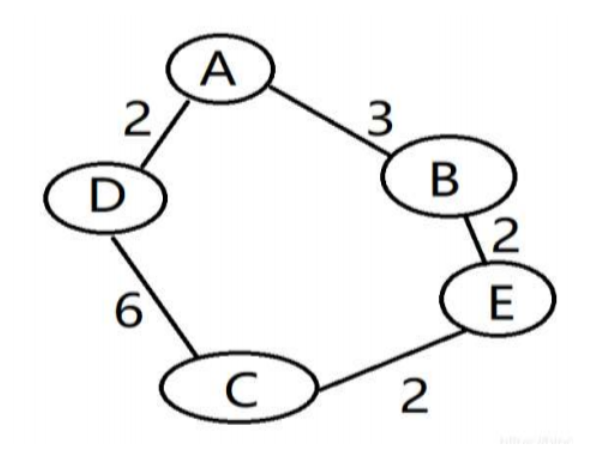
\includegraphics[width=0.45\linewidth]{images/UCS.png}
        \caption{UCS例}
        \label{fig:placeholder}
    \end{figure}
    {\small\kaishu
    \begin{itemize}
    \item \textbf{一致代价搜索执行过程：}设 $A$ 为起点，$C$ 为终点。frontier 为按路径代价从小到大排序的优先队列，explored 为已扩展状态集合。

    \begin{itemize}
        \item \textbf{初始化：}
        \[
        frontier=[A(0)],\qquad explored=\varnothing
        \]

        \item \textbf{第1步：}取出队首 $A(0)$，$A$ 不是目标，加入 explored，并扩展其后继 $D,B$：
        \[
        frontier=[D(2),\,B(3)],\qquad explored=\{A\}
        \]

        \item \textbf{第2步：}取出队首 $D(2)$，$D$ 不是目标，加入 explored，并扩展其后继 $C$：
        \[
        frontier=[B(3),\,C(8)],\qquad explored=\{A,D\}
        \]

        \item \textbf{第3步：}取出队首 $B(3)$，$B$ 不是目标，加入 explored，并扩展其后继 $E$：
        \[
        frontier=[E(5),\,C(8)],\qquad explored=\{A,D,B\}
        \]

        \item \textbf{第4步：}取出队首 $E(5)$，$E$ 不是目标，加入 explored，并扩展其后继 $C$。此时新路径
        \[
        A\to B\to E\to C
        \]
        的代价为
        \[
        3+2+2=7
        \]
        而 frontier 中原有 $C(8)$，由于 $7<8$，因此用更优的 $C(7)$ 替换原来的 $C(8)$：
        \[
        frontier=[C(7)],\qquad explored=\{A,D,B,E\}
        \]

        \item \textbf{第5步：}取出队首 $C(7)$，发现 $C$ 是目标，搜索成功：
        \[
        frontier=\varnothing,\qquad explored=\{A,D,B,E,C\}
        \]

        \item \textbf{最优路径：}
        \[
        A\to B\to E\to C
        \]
        \item \textbf{路径代价：}
        \[
        3+2+2=7
        \]
    \end{itemize}
\end{itemize}
    }
    \item \textbf{深度优先搜索（Depth-first Search, DFS）}
    \begin{itemize}
        \item \textbf{原理：}首先扩展未被扩展的节点中最深的那个
        \item \textbf{数据结构：}栈（LIFO）
        \item \textbf{过程：}优先级队列，插入队列时按代价值排序，取出队列中代价值最小的节点即头节点，遍历该节点子节点并插入合适位置，此次类推；
    \end{itemize}
    \item \textbf{有限深度优先搜索（深度受限搜索）（Depth-limited Search, DLS）}
    \item \textbf{迭代加深搜索（迭代加深的深度优先搜索）（Iterative Deepening Search, IDS / Iterative Deepening Depth-first Search, IDDFS）}
\end{enumerate}


\subsection{启发式搜索算法}\label{sec:heuristic-search}
\begin{enumerate}
    \item \textbf{贪婪最佳优先搜索}
    \begin{itemize}
        \item \textbf{思想：}在每一步扩展中，都要试图找到离目标最近的节点
        $$f(n)=h(n)$$
        \item \textbf{缺点：}
        \begin{itemize}
            \item 目前代价小，之后代价不一定小；
            \item 如果解在代价最大点，可能会找不到解进入死循环；
        \end{itemize}
    \end{itemize}
    \item \textbf{A*算法}
    \begin{itemize}
        \item \textbf{思想：}避免扩展代价昂贵的节点
                $$f(n)=g(n)+h(n)$$
        \item \textbf{启发式函数}
        \begin{itemize}
            \item \textbf{可容纳启发式：}如果$h$从不高估到达目标的最低路径耗散值\footnote{总是很乐观很理想的估计}，我们称$h$是admissible（可容纳的）
            \item \textbf{优劣比较：}如果对于所有的节点 \( n \) 有 \( \;{h}_{2}\left( n\right)  \geq  {h}_{1}\left( n\right) \) (都是可容许的)，则$h_2 $优于$ h_1$ 且更适于搜索\footnote{即估的越准越适合搜索。}
            \item \textbf{性能影响：}可用有效分支因子 $b^*$ 衡量启发式函数的质量。若 A* 共生成 $N+1$ 个节点（含起始节点），解深度为 $d$，则
            $$
            N+1=1+b^*+(b^*)^2+\cdots+(b^*)^d
            $$
            $b^*$ 越小，说明启发式越有效；$b^*$ 越接近 $1$，说明启发式越接近完美。  
            
            {\small\kaishu 例如，若 A* 用 $52$ 个节点在第 $5$ 层找到解，则 $b^*\approx 1.92$。}
        \end{itemize}
        \item \textbf{性质：}如果$h$是可容纳的，那么使用树搜索的A*算法是最优的\footnote{可用反证法证明。但如果用图搜索代替树搜索，则解有可能是非最优解。因为有重复状态而被丢弃，返回的解就是非最优的。}
        \item \textbf{缺点：}
        \begin{itemize}
            \item 处于目标等值线搜索空间内的节点数是解长度的指数函数
            \item 对存储空间要求很高，在内存空间中保存了所有的节点。
        \end{itemize}

        
    \end{itemize}

    \item \textbf{IDA*（迭代深入A*）}\footnote{这个名字我觉得起的很误导，理解一下：实际上就是DFS，但是DFS是无限往深搜。这里先介绍IDS，即迭代深入搜索（后面会有），相比于DFS它的改进是设置了一个深度阈值，一开始设为1，如果一层没搜到结果，那么阈值改为2，就最深搜到第二层，如果还不行就改为3，总之是到了第n层搜索就停止；进一步看IDA*，就是把深度阈值改为f阈值，仍然是按深度优先搜索，实际上搜索过程不是A*，即不是选f最小的那个，叫A*只是因为每一个节点都算了一下f值决定要不要停止搜索而已。这就是为什么说不需要判重，不需要排序，因为搜索根本不是按A*选择的。p.s.所以我觉得这课讲的顺序真的很神秘很诡异。}
    \begin{itemize}
        \item \textbf{动机：}A*对存储空间要求很高，因此需要减少存储要求：存储受限的启发式搜索
        \item \textbf{截断值：}$f$代价\footnote{普通的迭代加深算法截断值是搜索深度，而IDA*是$f$代价}
        \item \textbf{做法：}先给一个$ f $阈值；然后按深度优先往下搜；只要某个节点的$ f(n) $超过阈值，就直接剪掉，不继续展开；本轮没找到解，就把阈值提高，再来一轮 DFS。
        \item \textbf{优势：}
        \begin{itemize}
            \item 不需要判重，不需要排序
            \item 可以避免节点队列排序的实际系统开销，空间需求减少
        \end{itemize}
    \end{itemize}
\end{enumerate}
\textcolor{red}{下面这个表格能理解最好，理解不了就把时间空间复杂度背下来吧，考选择。}
以防有同学忘记：

完备性：如果有解一定能找到（比如DFS如果是个图的话可能一直死循环找不到可行解）
最优性：不是说算法最优，而是说能找到最优的解
\begin{center}
\renewcommand{\arraystretch}{1.2}
\begin{tabularx}{\textwidth}{>{\raggedright\arraybackslash}p{2.8cm}
>{\raggedright\arraybackslash}X
>{\raggedright\arraybackslash}X
>{\raggedright\arraybackslash}X
>{\raggedright\arraybackslash}X}
\toprule
算法 & 完备性 & 时间复杂性 & 空间复杂性 & 最优性 \\
\midrule
BFS
& Yes\footnote{要求分支因子 $b$ 有限。}
& $O(b^{d+1})$
& $O(b^{d+1})$
& Yes\footnote{要求每步耗散相同，通常取 $1$。} \\

UCS
& Yes\footnote{要求每步耗散存在正下界，即 $\ge \varepsilon > 0$。}
& $O\!\left(b^{1+\lfloor C^*/\varepsilon \rfloor}\right)$
& $O\!\left(b^{1+\lfloor C^*/\varepsilon \rfloor}\right)$
& Yes\footnote{要求每步耗散为正。} \\

DFS
& No
& $O(b^m)$
& $O(bm)$
& No \\

Greedy
& No\footnote{在有限状态空间中，若进行重复状态检测，则可完备。}
& $O(b^m)$
& $O(b^m)$
& No \\

A*
& Yes\footnote{除非存在无穷多个满足 $f(n)\le f(G)$ 的节点。}
& 指数级\footnote{通常随解深度呈指数增长。}
& 指数级\footnote{因为需要保存所有已生成节点。}
& Yes\footnote{当启发函数 $h(n)$ 可采纳时成立；树搜索版本最优。} \\

IDA*
& Yes\footnote{当启发函数 $h(n)$ 可采纳时成立。}
& 难以精确描述\footnote{取决于 $h(n)$ 的精确程度以及最优路径代价的增长方式。}
& $O(bd)$
& Yes\footnote{当启发函数 $h(n)$ 可采纳时成立。} \\
\bottomrule
\end{tabularx}
\end{center}

其中：
\begin{itemize}
    \item $b$：分支因子；
    \item $d$：最浅目标节点深度；
    \item $m$：状态空间最大深度；
    \item $C^*$：最优解路径耗散；
    \item $\varepsilon$：单步耗散的下界。
\end{itemize}



\subsection{局部搜索算法}\label{sec:local-search}

启发式搜索一般适用于：环境\textbf{可观察、确定、已知}，问题的解是一个\textbf{行动序列}，关注的是\textbf{路径代价}；而局部搜索更适用于那些\textbf{解与路径无关}的问题，即只关心最终达到的状态是否足够好，而不关心是怎样到达该状态的。局部搜索直接把\textbf{状态本身}作为优化对象。

可用来求解\textbf{连续空间}上的问题

因此，局部搜索的基本思想是：
\begin{itemize}
    \item 保持一个\textbf{当前状态}；
    \item 对当前状态进行评价；
    \item 不断移动到某个更优的邻近状态，试图改进当前解。
\end{itemize}

局部搜索通常\textbf{不保留完整路径}，只关心当前状态及其邻域，所以有以下特点：
\begin{itemize}
    \item \textbf{关注点：}解状态，而不是路径代价；
    \item \textbf{优点：}所需内存很少；
    \item \textbf{适用性：}常能在很大甚至无限的状态空间中找到合理解；
    \item \textbf{特点：}比传统路径搜索更接近现实中的优化问题。
\end{itemize}

\begin{enumerate}
    \item \textbf{爬山法}
    \begin{itemize}
        \item \textbf{思想：}即每次都在临近的空间中选择最优解作为当前解，直到局部最优解\footnote{模拟爬山的过程：随机选择一个位置爬山，每次朝着更高的方向移动，直到到达山顶}；
        \item \textbf{特点：}
        \begin{itemize}
            \item 简单的循环过程
            \item 采用启发式方法。
            \item 是对DFS的一种改进。
            \item 利用反馈信息帮助生成解的决策。
            \item 不会考虑与当前状态不相邻的状态，算法不维护搜索树，当前节点的数据结构只记录当前状态和目标函数值。
        \end{itemize}
        \item \textbf{缺点：}
        \begin{itemize}
            \item 算法会陷入局部最优解。
            \item 能否得到全局最优解取决于初始点的位置。
        \end{itemize}
        \item \textbf{举例：}八皇后问题
    \end{itemize}
    \begin{figure}[H]
        \centering
        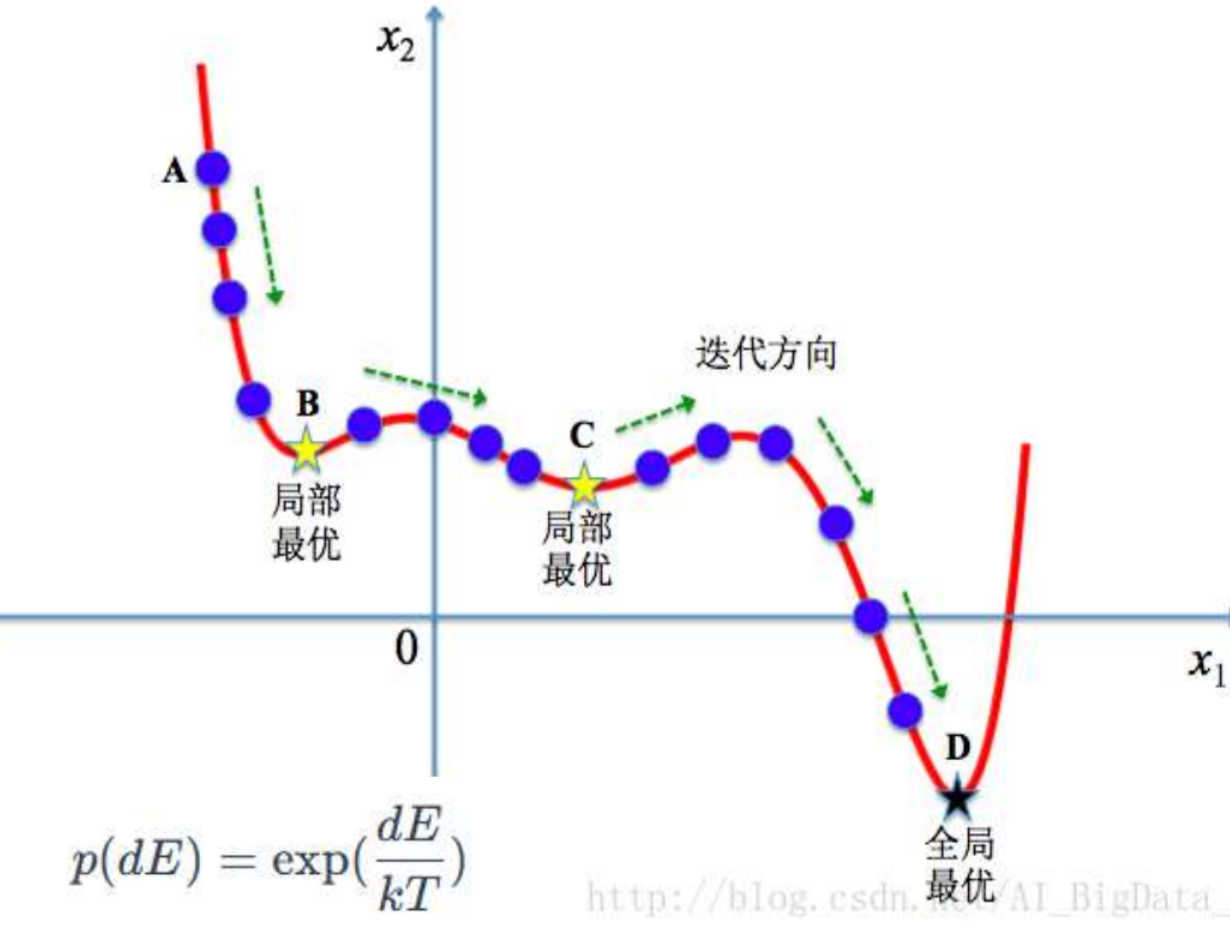
\includegraphics[width=0.5\linewidth]{images/monituihuo.png}
        \caption{模拟退火算法图示}
        \label{fig:placeholder}
    \end{figure}
    \item \textbf{模拟退火算法}：改进爬山法，允许一定概率接受“更差”的状态，以避免陷入局部极小点，同时兼顾搜索效率与全局寻优能力。
    \begin{itemize}
        \item \textbf{基本思想：}从当前状态出发，随机选择一个邻居；若邻居更优，则直接接受；若邻居更差，也以一定概率接受。
        
        \item \textbf{概率机制：}在温度 $T$ 下，状态被选中的概率服从 Boltzmann 分布：
        $$
        p(x)=\alpha e^{-\frac{E(x)}{kT}}
        $$
        其中：
        \begin{itemize}
            \item $E(x)$ 表示状态 $x$ 的能量，可理解为代价或目标函数值；
            \item $T$ 表示当前温度；
            \item $k$ 为常数；
            \item $\alpha$ 为归一化常数。
        \end{itemize}
        
        \item \textbf{对差解的接受规律：}若从当前状态移动到新状态导致能量增加 $\Delta E>0$，则仍可能接受该移动；并且：
        \begin{itemize}
            \item 温度越高，接受这类“更差移动”的概率越大；
            \item 温度越低，接受这类“更差移动”的概率越小。
        \end{itemize}
        
        \item \textbf{温度的作用：}
        \begin{itemize}
            \item \textbf{高温阶段：}搜索更随机，更容易跳出局部最优；
            \item \textbf{低温阶段：}搜索更稳定，更接近爬山法，只在局部做精细改进。
        \end{itemize}
        
        \item \textbf{性质：}若温度下降得足够缓慢，则算法达到全局最优状态的概率可趋近于 $1$。
    \end{itemize}
\end{enumerate}


\subsection{元启发式算法}\label{sec:metaheuristic}
    \begin{figure}[H]
        \centering
        
\includegraphics[width=0.75\linewidth]{images/yichuansuanfa.png}
        \caption{遗传算法图例}
        \label{fig:placeholder}
    \end{figure}
\begin{enumerate}
    \item \textbf{遗传算法}：保留大量状态种群的随机爬山法搜索，杂交和变异是算法的关键操作
    
    遗传算法将搜索结构编码为字符串形式，每个字符串称为一个\textbf{个体}，一组个体构成\textbf{种群}。算法不直接在参数本身上操作，而是在编码后的个体上进行选择、交叉、变异等操作，并根据适应度不断产生新一代种群。
    \begin{itemize}

    \item \textbf{基本思想：}
    \begin{itemize}
        \item 从 $k$ 个随机生成的状态开始，形成初始种群；
        \item 每个状态用一个有限长度的字符串表示，通常可写成 $0$-$1$ 串；
        \item 对每个个体计算评价值，称为\textbf{适应度}；
        \item 适应度高的个体有更大概率被保留下来并参与繁殖；
        \item 通过选择、交叉、变异产生下一代。
    \end{itemize}

    \item \textbf{基本流程：}
    \begin{enumerate}
        \item 将实际问题的目标函数映射为适应度函数；
        \item 对候选解进行编码，形成初始种群；
        \item 计算每个个体的适应度；
        \item 判断是否满足终止条件；若满足，则输出结果；
        \item 否则依次进行\textbf{选择}、\textbf{交叉}、\textbf{变异}；
        \item 生成新一代种群并继续迭代。
    \end{enumerate}

    \item \textbf{常用遗传算子：}
    \begin{itemize}
        \item \textbf{选择（selection）：}根据适应度选择较优个体进入下一步；
        \item \textbf{交叉（crossover）：}结合两个父状态的信息生成后继状态；
        \item \textbf{变异（mutation）：}对个体的局部编码做随机改变，以增加多样性；
        \item \textbf{复制（reproduction）：}直接保留较优个体；
        \item \textbf{反转（inversion）：}改变部分基因片段的顺序。
    \end{itemize}

    \item \textbf{与传统优化方法的区别：}
    \begin{itemize}
        \item 不直接作用在参数集上，而是作用于参数的某种编码；
        \item 不是从单个点开始搜索，而是从一个点的群体开始搜索\footnote{爬山法是最朴素的单点邻域贪婪搜索；模拟退火在爬山法的基础上加入概率接受劣解机制，因此既可视为局部搜索的升级版，也常因策略通用而被列为元启发式；遗传算法则彻底跳出单点邻域，用多点种群的交叉-变异-选择框架，成为最典型的元启发式代表}；
        \item 利用适应度信息，无须导数或其他辅助信息；
        \item 利用概率转移规则，而非确定性规则。
    \end{itemize}

    \item \textbf{优点：}
    \begin{itemize}
        \item 不容易陷入局部最优；
        \item 即使适应度函数不连续、非规则或含噪，也往往能找到较好的整体解；
        \item 具有天然并行性，适合并行计算。
    \end{itemize}

    \item \textbf{局限：}
    \begin{itemize}
        \item 解的质量依赖于编码方式、适应度函数和参数设置；
        \item 不能保证一定找到全局最优解；
        \item 收敛速度和稳定性在不同问题上差异较大。
    \end{itemize}

    \end{itemize}
\end{enumerate}
\end{document}
